\chapter{The Artificial Neural Network: YOLO-v3}
\label{ch:The Artificial Neural Network: YOLO-v3}

\section{Introduction}
The artificially generated multi-layer perceptron architecture is inspired by the biological neural structure of the human brain. It is identified as an artificial neural network (ANN), as it is structured with millions of connected nodes or called artificial neurons in a hierarchical pattern. In a neural network, millions of units are grouped in different layers to create a deep neural network to perform complex human-level functions. The ANN is an organized structure of different types of layers connected in a serial or parallel manner. To achieve a human-like performance, hundreds of layers are connected in a complex pattern to generate a deep neural network, and the empirical results summarized in \cite{goodfellow} prove that the ANN has the capability to perform tasks that are impossible by conventional algorithms.

In the fully connected layer of any neural network, all nodes of the preceding layer have connections with all the nodes in the next layer. The connection between nodes of two successive layers is identified as a signal. Each signal contains two parameters: weight and bias. The values of these parameters state the influence of one node on another. The weight and bias are the learn-able parameters that can be learned while training. These two quantities implicitly control the training evaluation that will be discussed in detail later in this chapter.

Mainly, the artificial neural network comprising an input layer, multiple hidden layers, and an output layer. As shown in Fig. \ref{ANN_Arch} the input layer contains the training dataset such as images for the classification problem, audio clips for speech recognition, and labeled image datasets for object detection problems. The convolutional neural network can only accept image data in the input layer whereas the recurrent neural network only takes time-series data. The hidden layers contain multiple groups of layers such as a fully connected layer, convolutional layer, normalization layer, Relu activation layer, sigmoid activation layer, pooling layer, and many more. Finally, the output layer is a classification layer based on the function of ANN. Therefore, it can be a SoftMax layer for multi-class classification or a binary classification layer for identifying a single class object.

\begin{figure}
    \centering
    \fbox { 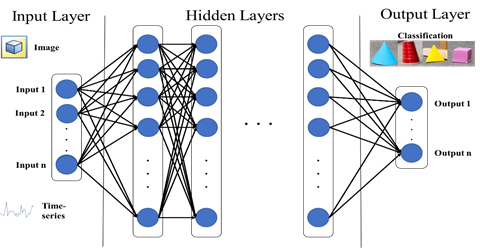
\includegraphics[scale= 0.8]{Images/ANN_Architecture.png}}
    \caption{Artificial Neural Network Architecture}
    \label{ANN_Arch}
\end{figure}

\section{YOLO-v3 Architecture}
The YOLO-v3 network is a concatenation of a convolutional neural network (CNN) and multiple detection heads \cite{yolov3}. In this architecture, CNN is used for feature detection and image classification, and multiple detection heads are used to localize and detect an object in a frame. More than one detection heads are used to detect the various size of objects. The bigger sized head can detect a tiny object or the object positioned far from the camera and vice versa. This type of structure can be created by using any efficient convolutional neural network with any number of detection heads by considering the computational cost of time delay in response. This architecture uses anchor box estimation of labeled training data to accurately predict the bounding box. 

This network uses YOLO (you only looks once) algorithm to localize and detect the object. Unlike the conventional detection algorithm (the sliding window algorithm), the YOLO algorithm divides the input image into grids and localizes objects within a frame. In terms of computational speed, the YOLO proves to be faster than its counterparts such as R-CNN, Fast-RCNN, and Faster-RCNN networks \cite{yolov3}. These networks use the variances of the sliding window algorithm. The YOLO detection algorithm will be explained in detail later in this chapter. 

\begin{figure}
    \centering
    \fbox {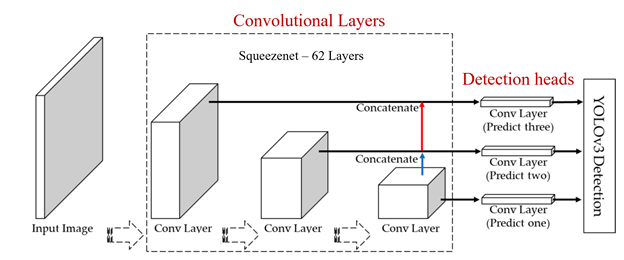
\includegraphics[width=0.95\textwidth,height=2.5in]
    {Images/layersYOLO.png}}
    \caption{Stacks of Layers in YOLO-v3 Network \cite{rs12010044}}
    \label{Layers}
\end{figure}

The YOLO-v3 architecture is pictured in Fig. \ref{Layers}. The input layer contains the training data as a labeled image dataset. The input layer image size is defined as 227×227×3. Therefore, this network accepts RGB images of size 227×227. In the input layer before passing the image dataset to the successive layer, all images are resized to column vectors of size 154587×1. The column vectors of a dataset of a total of 8600 images are then concatenated in a large matrix of size 154587×8600. The hidden layers comprise convolutional layers grouped with non-linear activation layers such as Relu, sigmoid, and hyperbolic tangent layer. The size of the convolutional layer becomes smaller as moving deeper into the network. Three different sizes of activations from the convolution layer taken as input for the detection heads. The three-detection heads, of various sizes in the given case, are used to detect the different sizes of objects. The size of the detection head is pre-determined on what size of the object the network requires to detect. At the output layer, the detection head gives a class of objects, bounding box coordinates, and precision in output for each detected object.

\section{Layers in Neural Network Architecture}
The artificial neural network, as mentioned earlier in this chapter, is a stack of an organized group of various types of layers. All these layers are grouped systematically to accomplish the purpose of the network. Besides, the non-linear activation functions are grouped to pose non-linearities in the results, which is important when data does not follow the uniform distribution. The types of layers in the neural networks are explained in detail below. 

\subsection{Input Layer}
The input layer takes grayscaled or RGB images to a network for object classification or detection problems. In this layer, the size of the input image is pre-defined at the time of neural network design and it can not be modified in the case of transfer learning \cite{coursera1}. The primary purpose of the input layer is to filter the images that match the size with the input layer. This layer does not perform any computation other than feeding the dataset to the hidden layers.

\subsection{Convolutional Layer}
The convolutional layer is the main building block of the convolutional neural network. In this layer, the convolutional operations are performed over the set of images to detect features such as edges, textures, patterns, parts, and objects. To perform the convolution operation, the size parameters of the convolutional filter such as height, width, and depth are defined as per the requirements. The depth of the filter is the same as the number of channels of the input image in the majority of cases and it trains to detect a single feature of the input dataset. In the backpropagation in supervised learning, the weight parameters of the filter are learned unless required accuracy can be acquired and then stored in the respective layers of the network for the further application. 

In the convolution operation, each weight parameter of the filter dot multiplied with each respective pixel of the image, and then all results were summed together. By sliding the filter horizontally and vertically simultaneously and applying dot multiplication to respective entries of the filter and input image to generate an activation that passes to the upcoming layer. The convolution operation is graphically represented in Fig. \ref{convope}, where the input image size is 227×227×3, and the filter size is 3×3×3. After the convolutional operation, the output size became 225×225×3. Therefore, it seems that at each convolution layer, the size of the image gets reduce as it passes deeper into the network.  
     
\begin{figure}
    \centering
    
    \begin{subfigure}[]
        \centering
        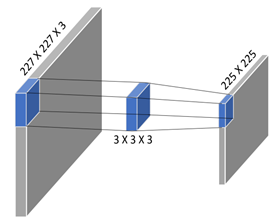
\includegraphics[width=0.4\textwidth]{Images/conv1l.png}
    \end{subfigure}
    % \rule{1px}{140px}
    \begin{subfigure}[]
        \centering
        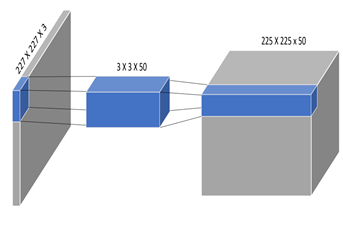
\includegraphics[width=0.5\textwidth]{Images/convmultil.png}
    \end{subfigure}
 
    \caption{Convolution operation over (a) a single filter and (b) multi-filters}
    \label{convope}
\end{figure}    
     
Each layer of the convolutional neural network is predefined with the number of features its needs to detect. Since each convolution filter can detect a single feature from the input image, it needs to define the same number of filters as the number of features needs to detect. The outcomes from each filter are concatenated into a multi-channel activation. For instance, an image of size 227×227×3 is passing from a Conv layer having 50 filters as depicted in \ref{convope}(b), the output will be of the size 225×225× 50. 

The size of activation from the Conv layer can be controlled by three hyper-parameters: 1. Number and size of filters, 2. Padding size, and 3. Stride length. 

\textbf{1.	Filter size and numbers:}
The filter width and height are selected by considering the proportion of data association requires between the conv filter and the input image. The larger size in width and height of the filter represents the greater amount of data association, however, the outcome became shorter. The relationship between input size, filter size, and the output size is defined as follows. 

\begin{equation} \label{eq1}
n^{[L]}=n^{[L-1]}-f+1
\end{equation}

where, $n^{[L]}$S is output size, $n^{[L-1]}$ is input size, $f$ is filter size and $L$ is the layer number.

As per the Eq. (\ref{eq1}), the depth of the outputs is governed by the number of filters used in the conv layer and Input image size. Therefore, the size of the depth is similar to the number of filters. For instance, if the Conv layer of $n_f$ filters having the size $f \times f \times n_c^{[L-1]}$  and the size of an input image is $n_w^{[L-1]} \times n_H^{[L-1]} \times n_c^{[L-1]}$, the size of the output becomes $(n_w^{[L-1]} - f+1) \times (n_H^{[L-1]} - f+1) \times n_f$.

\textbf{2.	Padding:}
There are two disadvantages of the Conv network. The first is at each Conv layer, the size of the image decreases, and the second is the pixel values at the edge of the image are not associated with multiple values in the activation, because of this the important information at the edge is ignored. For the deep neural network that has a hundred or more than a hundred Conv layers, the reduction in the size of the image is not acceptable. 

To overcome these disadvantages, the padding is applied at each edge of the input image as illustrated in Fig. \ref{Padding}. The border of the input image is padded with zeros such that the output size becomes the same as the original input size. Such type of convolution operation is known as “the same convolution”, and without padding is identified as “the valid convolution”. The relation between output and input size is as follows.

\begin{equation} \label{eq2}
n^{[L]}=n^{[L-1]}+2p-f+1
\end{equation}

where, $p$ is padding, and $f$ is filter's size

\textbf{3.	Stride:}
The stride length is defined as how many pixels need to skip while sliding the filter over the input image. In general, the stride length is 1, which means the filter slides over each pixel in the image. As represented in Fig. \ref{Padding}, in the Conv layer with stride length 2, the filter jumps to 2 pixels and it skips the pixel at the middle position. If the value of the stride length for any Conv layer is more than one, the relation of output and input is defined as follows. 

\begin{equation}
n^{[L]}=\frac{n^{[L-1]}+2 p-f}{S}+1
\end{equation}

\begin{figure}
    \centering
    \fbox {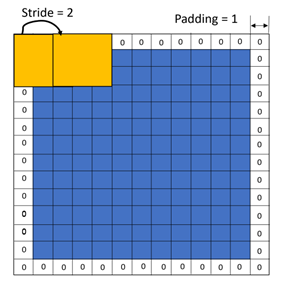
\includegraphics[width=0.55\textwidth]
    {Images/padding.png}}
    \caption{Stride and Padding in the Conv Layer}
    \label{Padding}
\end{figure}

To combine all hyper-parameters, if the filter size is $f^{[L]}$ , padding of size $P^{[L]}$ , stride length $s^{[L]}$ , number of filters $n_C^{[L]}$ , input image size $n_H^{[L-1]} \times n_w^{[L-1]} \times n_c^{[L-1]}$ , and the output size is $n_H^{[L]} \times n_w^{[L]} \times n_c^{[L]}$ 

\begin{itemize}
\item Each filter dimension is $f^{[L]} \times f^{[L]} \times n_c^{[L-1]}$.
\item Activation size is $n_H^{[L]} \times n_w^{[L]} \times n_c^{[L]}$.
\item The total number of weights are $f^{[L]} \times f^{[L]} \times n_c^{[L-1]} \times n_c^{[L]}$.
\item The total number of bais is $n_c^{[L]}$. 
\end{itemize}

\subsection{Non-linear Activation Layer}
The non-linear activation layer is used just after the Conv layer. The feature map generated by the conv layer is taken as input and generates an activation map in output. Since the operation in this layer is performed element-wise, the output dimensions are similar to input dimensions. 

The function of this layer is to impose low-level non-linearity into the feature map created by the conv layer. Since the conv layer operation is a linear function, the network without any nonlinear activation layer generates a linear classifier that has a high bias value. The trained neural network with high bias is not acceptable in any practical application. Fig. \ref{activation} illustrates the difference between linear and non-linear classifiers on a sample dataset. 

\begin{figure}
    \centering
    \fbox {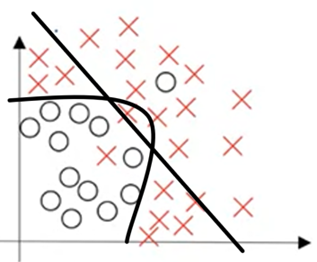
\includegraphics[width=0.55\textwidth]
    {Images/activation.png}}
    \caption{The shape of the classifier of the neural network with and without non-linear activation \cite{coursera1}}
    \label{activation}
\end{figure} 

There are many types of activation functions used in the non-linear layer such as sigmoid, hyperbolic tangent, Relu (rectified linear unit), and leaky Relu. The illustration of these activation functions is shown in Fig. \ref{activations}. 

\begin{figure}
    \centering
    
    \begin{subfigure}[]
        \centering
        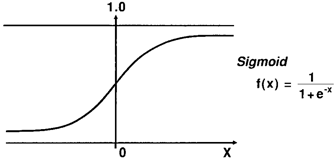
\includegraphics[width=0.45\textwidth]{Images/sigmoid.png}
    \end{subfigure}
    \rule{1px}{100px}
    \begin{subfigure}[]
        \centering
        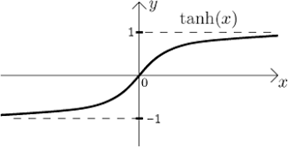
\includegraphics[width=0.45\textwidth]{Images/hypertan.png}
    \end{subfigure}
    \rule{\textwidth}{1pt}
     \begin{subfigure}[]
        \centering
        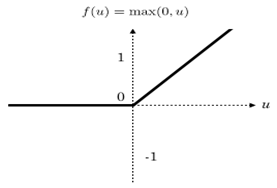
\includegraphics[width=0.45\textwidth]{Images/relu.png}
    \end{subfigure}
    \rule{1px}{120px}
    \begin{subfigure}[]
        \centering
        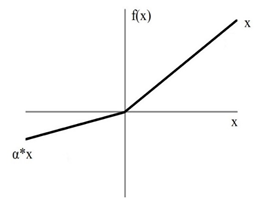
\includegraphics[width=0.45\textwidth]{Images/leakyrelu.png}
    \end{subfigure}   
    
    \caption{Non-linear Activation functions (a) Sigmoid, (b) Hyperbolic tangent, (c) Relu, and (d) Leaky Relu function \cite{coursera1}}
    \label{activations}
\end{figure} 

The sigmoid and hyperbolic tangent functions are the exponential functions. The sigmoid function varies from 0 to 1, and the hyperbolic tangent function varies from -1 to 1. As illustrated in Fig. \ref{activations} (a) and (b), the mean of data of the sigmoid activation function is 0.5, and for the hyperbolic tangent function is 0. Therefore, the tangent activation function is superior to sigmoid activation and preferable for the hidden layers. However, the sigmoid activation is preferable when 0 or 1 require at the output in the case of binary classification. Both functions have a little change in the slop at the larger value of the input, and because of this, the learning process slows down. To overcome this issue, the rectified linear unit function is used. The rectified linear unit function has a slop value of 1 for 0 to 1 and for the rest of the part, it is 0 as seen in Fig. \ref{activations} (c). This activation function is also identified as Relu activation. The Relu has a non-zero value at 0, and it is a very small value such as 0.00000001. Since it has a constant slope, comparatively it is faster than the sigmoid and tangent activation. The improved version of Relu is leaky Relu activation that has a non-zero and little slope for the negative inputs as shown in Fig. \ref{activations} (d). In comparison, the Relu activation is preferable because of its faster learning speed. However, other activation functions are also used based on the purpose of the neural network.       

\subsection{Pooling or Down-sampling Layer}
The Pooling or Down-sampling layer extracts the most significant number by the predefined size of the window. Similar to the conv layer, the filter slides over each channel of the input image and reduces the size of the input. Therefore,  the pooling layer is used after several stages of conv layers or non-linearity layers to reduce the computational load, increase the speed of the training process, and prevent overfitting. The essential intuition behind the pooling layer is to discard the less significant data with preserving the main features of the image (for image recognition task) to reduce the cost due to the spatial resolution.  

The hyperparameters of this layer are filter size, stride length, and padding, however, the filter has no parameters that need to learn while training. The shape of the filter should not be required to be square, it can be parameterized to the size of the rectangle. However, it is rarely be used in the practice. Since the pooling process is performed in each channel, the size reduction is happening in width and height, and the depth size is always similar to the input size as demonstrated in Fig. \ref{downsample}. The most common type of pooling layer has a filter size of 2 X 2 and a stride length of 2. Such a type of pooling layer does not have any overlapping nature of the filter, so it filters the unique set of the data in the output. In contrast, if the stride length is less than the filter size, data in the middle of the channel of the image filter multiple times. This type of pooling layer is also known as an overlapping pooling layer. It is highly preferable to use an overlapping pool layer since it is proven to be used to prevent overfitting of the network. The larger filter size in the pooling layer has a destructive nature and degrades the performance of the neural network. 

\begin{figure}
    \centering
    \fbox {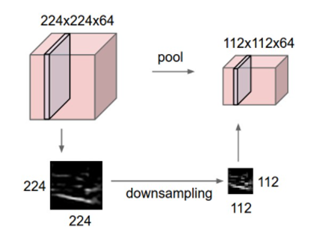
\includegraphics[width=0.6\textwidth]{Images/downsample.png}}
    \caption{The Pooling or Down-sampling Layer \cite{computersciencewiki}}
    \label{downsample}
\end{figure} 

There are two most common methods for the pooling layer. 

\begin{enumerate}
    \item Max Pooling
    \item Average Pooling
\end{enumerate}

In the max pooling, it extracts the maximum value from the predefined sized window region of the input image. On other hand, the average pooling finds the mean value from the window region. In terms of performance, the max-pooling seems faster and has better convergence compare to average pooling. 

\subsection{Up-sample Layer}
The Up-sampling layer is used when it needs to recover the input image or a part of the input image somewhere between the few Conv layer from the beginning and the output layer. The Up-sample layer converts the low-resolution image into a high-resolution image. This process can be done by learnable parameters or interpolation. Therefore, this layer can be defined with learnable parameters or non-learnable operations. In the interpolation, the elements in the small-sized input interpolated in multiple stages or row and column are copied many times. The learnable parameter is defined in the form of the elements of a predefined sized filter similar to the conv layer. However, unlike the conv network, the parameters get learned that generates an output that closely represents the ground truth image. The up-sampling can also be done by using “skip-connections”. It means that instead of taking input from the very last layer, it can be imported from any sallow layer that has a comparatively higher resolution. As a result,  the output accurately represents the ground truth image. 
In
The up-sampling layer is used in a task when a high resolution of the image is required, such as object localization and detection. For object localization, detection, and track tasks require high-resolution input to accurately predict the position of any object. However, the bigger size image slows down the processing time in the live detection problem. Therefore, to trade off between the processing time and accuracy, the input for the up-sample layer should be selected with enough resolution by using skip connections. The comparison of up-sampling outcomes from inputs from various layers is shown in figure \ref{upsample}.

\begin{figure}
    \centering
    \fbox {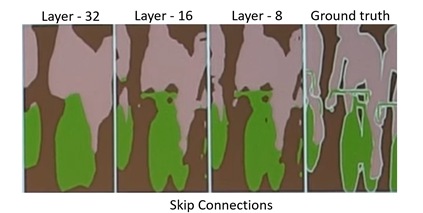
\includegraphics[width=0.6\textwidth]{Images/upsampling.png}}
    \caption{Up-sampling of inputs from various layers \cite{coursera1}}
    \label{upsample}
\end{figure}

\subsection{Fully Connected Layer}
The fully connected layer is usually located between the convolution layer and the output layer. The purpose of this layer is to combine all the features detected by the conv layers and generate a classification score for each class. The activation from the conv layer first flattens before considering it as input to the fully connected layer. All the elements of the activation from the conv layer are connected with each unit of the fully connected layer. Since each connection between units of fully connected layers posses weight property, the number of trainable parameters in this layer is much more than other conv layers in the convolutional neural network. However, the fully connected layer is not used in the YOLO-v3 architecture to increase the robustness in real-time object detection problems, as it contains many trainable parameters that reduce the overall performance.    

\begin{figure}
    \centering
    \fbox {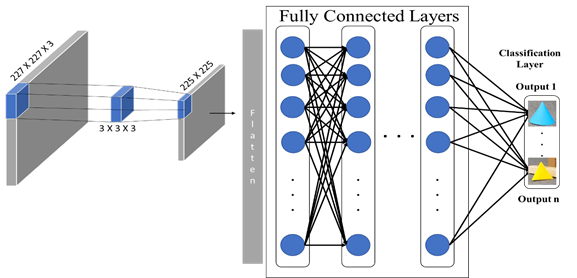
\includegraphics[width=0.6\textwidth]
    {Images/fullyconnected.png}}
    \caption{Fully Connected layers}
    \label{fullyconnected}
\end{figure}